% pdflatex pipeline.tex && pdftocairo -svg pipeline.pdf pipeline.svg
\documentclass[tikz,border=6pt]{standalone}
\usepackage[T1]{fontenc}
\usepackage{lmodern}
\usetikzlibrary{arrows.meta,positioning,fit,shapes.geometric,backgrounds,calc,shadows}
\pgfdeclarelayer{page}
\pgfsetlayers{page,background,main}

\begin{document}
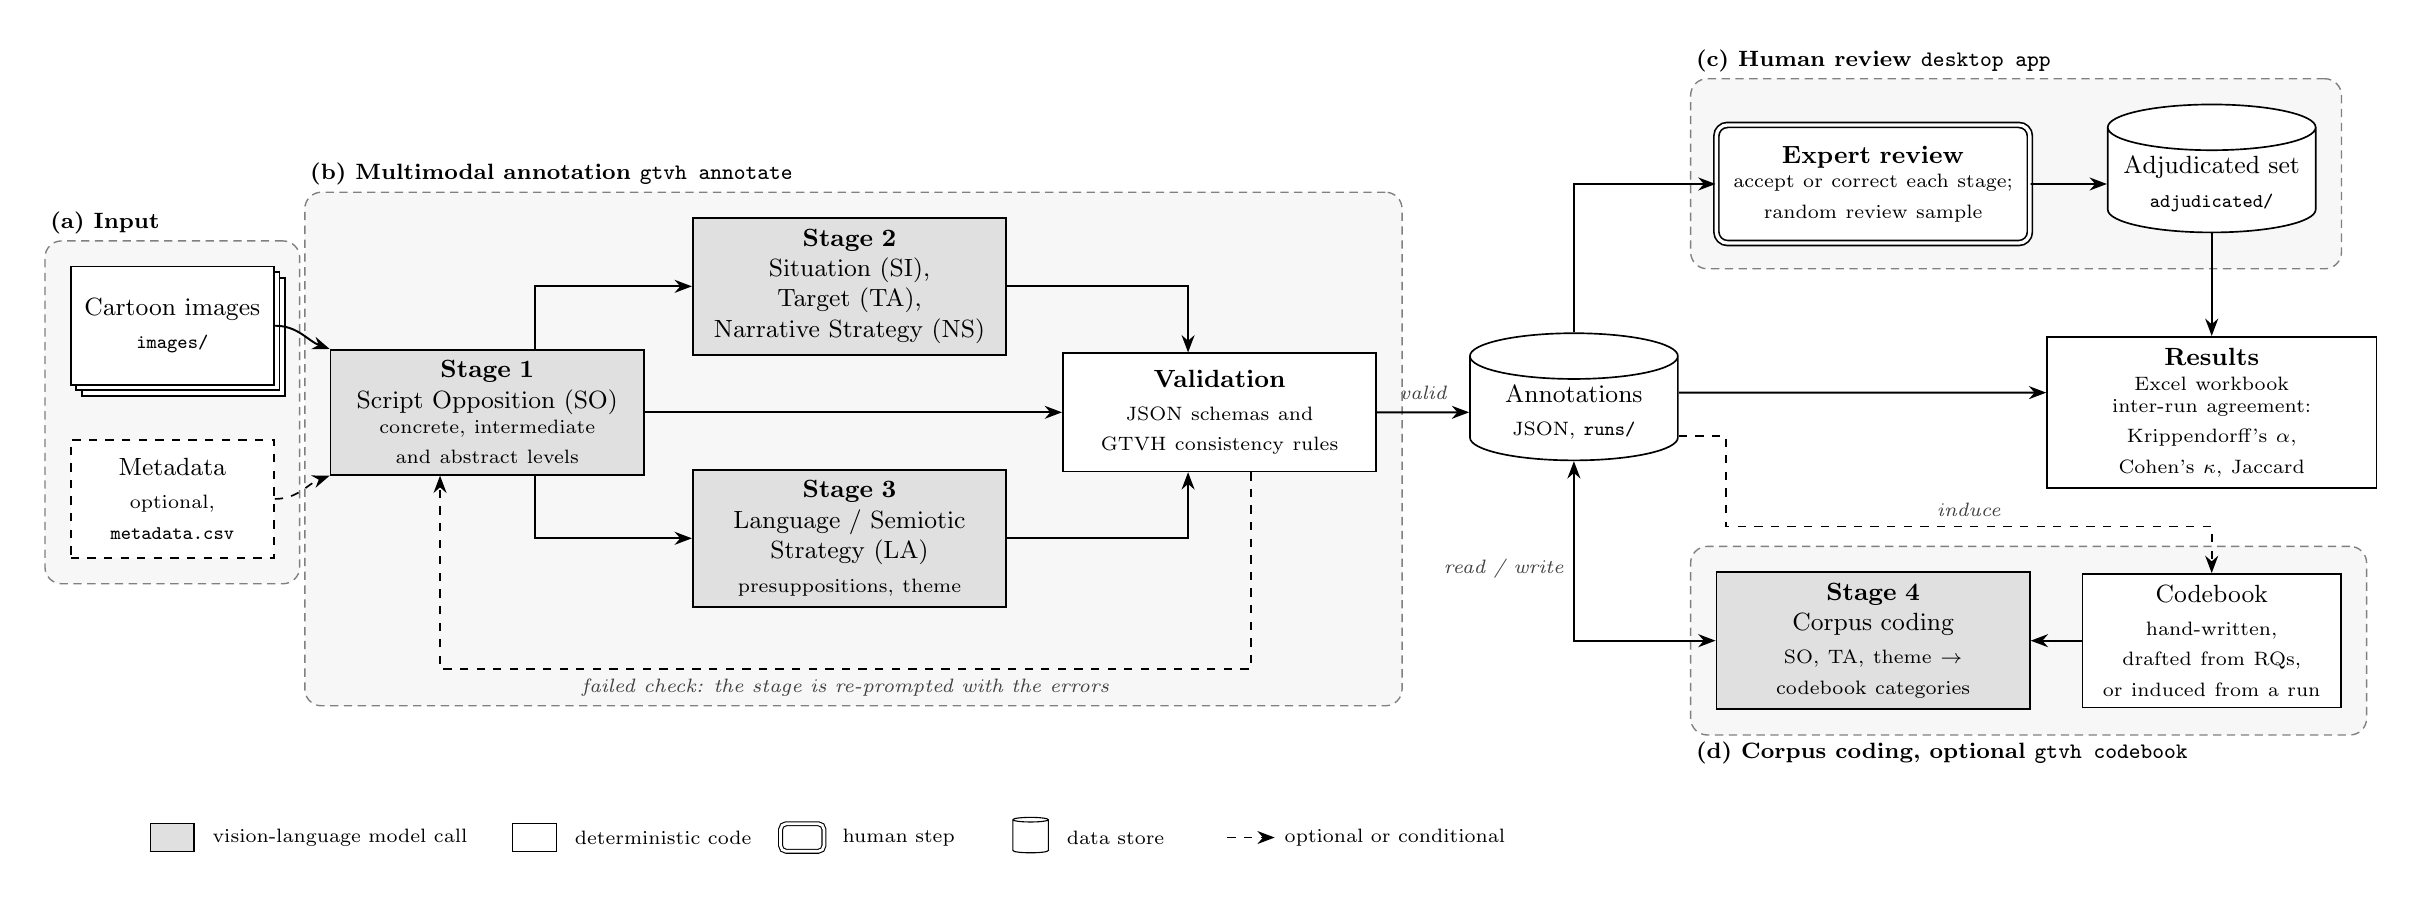
\begin{tikzpicture}[
    font=\small,
    >={Stealth[length=2.2mm]},
    every node/.style={align=center},
    base/.style={draw, line width=0.6pt, minimum height=1.5cm, inner sep=4pt,
                 execute at begin node={\hyphenpenalty=10000}},
    model/.style={base, fill=black!12, text width=3.7cm},
    code/.style={base, fill=white, text width=3.7cm},
    human/.style={base, fill=white, double, double distance=1.2pt, rounded corners=4pt, text width=3.7cm},
    store/.style={draw, line width=0.6pt, fill=white, cylinder, shape border rotate=90, aspect=0.22,
                  minimum height=1.5cm, text width=2.5cm, inner sep=2pt},
    file/.style={base, fill=white, text width=2.3cm},
    flow/.style={->, line width=0.7pt},
    aux/.style={->, line width=0.6pt, dashed},
    phase/.style={draw=black!50, line width=0.5pt, dash pattern=on 3pt off 2pt, rounded corners=6pt,
                  inner sep=9pt, fill=black!3},
    plabel/.style={font=\footnotesize\bfseries, anchor=south west, inner sep=2pt},
    note/.style={font=\scriptsize\itshape, text=black!75}
  ]

  \node[file, double copy shadow={shadow xshift=2pt, shadow yshift=-2pt}] (img) at (0, 1.1)
        {Cartoon images\\[1pt]\scriptsize\texttt{images/}};
  \node[file, dashed] (meta) at (0,-1.1)
        {Metadata\\[1pt]\scriptsize optional, \texttt{metadata.csv}};

  \node[model] (s1) at (4.0, 0)
        {\textbf{Stage 1}\\Script Opposition (SO)\\[1pt]\scriptsize concrete, intermediate\\and abstract levels};
  \node[model] (s2) at (8.6, 1.6)
        {\textbf{Stage 2}\\Situation (SI), Target (TA),\\Narrative Strategy (NS)};
  \node[model] (s3) at (8.6,-1.6)
        {\textbf{Stage 3}\\Language / Semiotic Strategy (LA)\\[1pt]\scriptsize presuppositions, theme};
  \node[code] (val) at (13.3, 0)
        {\textbf{Validation}\\[1pt]\scriptsize JSON schemas and GTVH consistency rules};

  \node[store] (runs) at (17.8, 0) {Annotations\\[1pt]\scriptsize JSON, \texttt{runs/}};

  \node[human] (rev) at (21.6, 2.9)
        {\textbf{Expert review}\\[1pt]\scriptsize accept or correct each stage;\\random review sample};
  \node[store] (adj) at (25.9, 2.9) {Adjudicated set\\[1pt]\scriptsize\texttt{adjudicated/}};

  \node[model] (s4) at (21.6,-2.9)
        {\textbf{Stage 4}\\Corpus coding\\[1pt]\scriptsize SO, TA, theme $\rightarrow$ codebook categories};
  \node[file, text width=3.0cm] (cb) at (25.9,-2.9)
        {Codebook\\[1pt]\scriptsize hand-written, drafted from RQs, or induced from a run};

  \node[code, text width=3.9cm] (res) at (25.9, 0)
        {\textbf{Results}\\[1pt]\scriptsize Excel workbook\\inter-run agreement:\\Krippendorff's $\alpha$, Cohen's $\kappa$, Jaccard};

  \draw[flow] (img.east) to[out=0, in=160] (s1.north west);
  \draw[aux]  (meta.east) to[out=0, in=200] (s1.south west);
  \draw[flow] ($(s1.north)+(0.6,0)$) |- (s2.west);
  \draw[flow] ($(s1.south)+(0.6,0)$) |- (s3.west);
  \draw[flow] (s1.east) -- (val.west);
  \draw[flow] (s2.east) -| ($(val.north)+(-0.4,0)$);
  \draw[flow] (s3.east) -| ($(val.south)+(-0.4,0)$);
  \draw[aux]  ($(val.south)+(0.4,0)$) -- ++(0,-2.5) -| node[note, pos=0.25, below] {failed check: the stage is re-prompted with the errors} ($(s1.south)+(-0.6,0)$);
  \draw[flow] (val.east) -- node[note, above=1pt] {valid} (runs.west);

  \draw[flow] (runs.north) |- (rev.west);
  \draw[flow] (rev.east) -- (adj.west);
  \draw[flow] ($(runs.east)+(0,0.25)$) -- ($(res.west)+(0,0.25)$);
  \draw[flow] (adj.south) -- (res.north);
  \draw[flow, <->] (runs.south) |- node[note, pos=0.3, left] {read / write} (s4.west);
  \draw[flow] (cb.west) -- (s4.east);
  \draw[aux]  ($(runs.east)+(0,-0.3)$) -| ++(0.6,-1.15) -| node[note, pos=0.25, above] {induce} (cb.north);

  \begin{scope}[on background layer]
    \node[phase, fit=(img)(meta)] (pa) {};
    \coordinate (loop) at ($(val.south)+(0,-2.65)$);
    \node[phase, fit=(s1)(s2)(s3)(val)(loop)] (pb) {};
    \node[phase, fit=(rev)(adj)] (pc) {};
    \node[phase, fit=(s4)(cb)] (pd) {};
  \end{scope}
  \node[plabel] at (pa.north west) {(a) Input};
  \node[plabel] at (pb.north west) {(b) Multimodal annotation \normalfont\texttt{gtvh annotate}};
  \node[plabel] at (pc.north west) {(c) Human review \normalfont\texttt{desktop app}};
  \node[plabel, anchor=north west] at (pd.south west) {(d) Corpus coding, optional \normalfont\texttt{gtvh codebook}};

  \begin{scope}[shift={(0,-5.4)}, every node/.style={font=\scriptsize, align=left}]
    \node[draw, fill=black!12, minimum width=0.55cm, minimum height=0.35cm] (l1) at (0,0) {};
    \node[right=3pt of l1] {vision-language model call};
    \node[draw, fill=white, minimum width=0.55cm, minimum height=0.35cm] (l2) at (4.6,0) {};
    \node[right=3pt of l2] {deterministic code};
    \node[draw, double, double distance=1pt, rounded corners=2pt, minimum width=0.55cm, minimum height=0.35cm] (l3) at (8.0,0) {};
    \node[right=3pt of l3] {human step};
    \node[draw, cylinder, shape border rotate=90, aspect=0.25, minimum width=0.45cm, minimum height=0.45cm] (l4) at (10.9,0) {};
    \node[right=3pt of l4] {data store};
    \draw[aux] (13.4,0) -- ++(0.6,0) node[right] {optional or conditional};
  \end{scope}

  \begin{pgfonlayer}{page}
    \fill[white] ([shift={(-6pt,-6pt)}]current bounding box.south west)
      rectangle ([shift={(6pt,6pt)}]current bounding box.north east);
  \end{pgfonlayer}
\end{tikzpicture}
\end{document}
